\documentclass{IFES-beamer}

% --------------------------------------------------- %
%           Información de la Presentación	          %
% --------------------------------------------------- %
\title[Pruebas con LaTeX Beamer]{Pruebas con LaTeX Beamer}
\subtitle{Actividad de Ejemplos y Ejercicios}
\author{Dylan Rodas}
\institute[UNIS]{
  Universidad del Istmo de Guatemala\\
  Facultad de Ingeniería
}
\date{30 de Noviembre, 2018}
\logo{

\includegraphics[scale=0.5]{Resources/Logo_UNIS.png}
}
\subject{Prácticas de Trabajo e Investigación 4}

% --------------------------------------------------- %
%             Título + Tabla de Contenidos            %
% --------------------------------------------------- %

\begin{document}

\begin{frame}
  \titlepage
\end{frame}

\begin{frame}{Contenido}
  \tableofcontents
\end{frame}

% --------------------------------------------------- %
%                      Presentación                   %
% --------------------------------------------------- %
\section{Múltiples Columnas}
\begin{frame}{Múltiples Columnas}

\begin{columns}
\begin{column}{0.5\textwidth}
Esto es la primera columna con muchas letras sin sentido. asdfghjklñ qwertyuiop zxcvbnm. y una imagen: 
\includegraphics[scale=0.25]{Resources/Tigre.jpg}
\end{column}
\begin{column}{0.5\textwidth}
Esto es la segunda columna con más letras sin sentido. ñlkjhgfdsa poiuytrewq mnbvcxz. y una imagen volteada: 
\includegraphics[scale=0.25, angle=180]{Resources/Tigre.jpg}
\end{column}
\end{columns}

\end{frame}

\section{Resaltar Texto}
\begin{frame}{Resaltar Texto}

Esto es Texto normal. \\
\alert{Esto es Texto de Alerta}. \\
\exemple{Esto es Texto de Ejemplo}. \\
\emph{Esto es Texto de Énfasis}. \\\

Debo \emph{enfatizar} que esto es un punto \alert{importante}. \\\

\textbf{Texto en negrita}.
\textit{Texto en italica}.
\textcolor{red}{Texto rojo}.
\textcolor{green}{Texto verde}.

\end{frame}

\section{Figuras}
\begin{frame}{Ejemplo de Figuras}

\begin{figure}
\centering

\includegraphics[scale=0.25]{Resources/Tigre.jpg}
\caption{Imagen de Ejemplo de \href{https://github.com/Rodas171315/PTI_4-DylanR-LaTeX_Beamer}{Github} PTI 4.}
\end{figure}

\end{frame}

\section{Tablas}
\begin{frame}{Ejemplo de Tablas}

\begin{columns}
  \begin{column}{0.5\textwidth}  

  \begin{tcolorbox}[tablegreen,tabularx={X||Y|Y}, boxrule=0.5pt, title=Tabla Verde]
  Columna 1 & Columna 2  & Columna 3 \\\hline\hline
  Fila 1    &   Item 1   &  Item 2   \\\hline
  Fila 2    &   Item 3   &  Item 4   \\\hline
  Fila 3    &   Item 5   &  Item 6    \\\hline\hline
  Fila 4    &   Item 7   &  Item 8 
  \end{tcolorbox}
  
  \begin{tcolorbox}[tablegrey,tabularx={X||Y|Y}, boxrule=0.5pt, title=Tabla Gris]
  Columna 1 & Columna 2  & Columna 3 \\\hline\hline
  Fila 1    &   Item 1   &  Item 2   \\\hline
  Fila 2    &   Item 3   &  Item 4   \\\hline
  Fila 3    &   Item 5   &  Item 6    \\\hline\hline
  Fila 4    &   Item 7   &  Item 8 
  \end{tcolorbox}
  
  \end{column}

  \begin{column}{0.5\textwidth}
  
  \begin{tcolorbox}[tableblue,tabularx={X||Y|Y}, boxrule=0.5pt, title=Tabla Azul]
  Columna 1 & Columna 2  & Columna 3 \\\hline\hline
  Fila 1    &   Item 1   &  Item 2   \\\hline
  Fila 2    &   Item 3   &  Item 4   \\\hline
  Fila 3    &   Item 5   &  Item 6    \\\hline\hline
  Fila 4    &   Item 7   &  Item 8 
  \end{tcolorbox}
  
  \begin{tcolorbox}[tableblack,tabularx={X||Y|Y}, boxrule=0.5pt, title=Tabla Negra]
  Columna 1 & Columna 2  & Columna 3 \\\hline\hline
  Fila 1    &   Item 1   &  Item 2   \\\hline
  Fila 2    &   Item 3   &  Item 4   \\\hline
  Fila 3    &   Item 5   &  Item 6    \\\hline\hline
  Fila 4    &   Item 7   &  Item 8 
  \end{tcolorbox}
  
  \end{column}
\end{columns}

\end{frame}

\section{Bloques}
\begin{frame}{Tipos de Bloques}

\begin{block}{Bloque Simple}
\begin{itemize}
  \item Simple.
  \item Simple.
  \item Y más simple.
\end{itemize}
\end{block}

\begin{exampleblock}{Bloque de Ejemplo}
\begin{itemize}
  \item Ejemplos.
  \item Ejemplos.
  \item Y más ejemplos.
\end{itemize}
\end{exampleblock}

\begin{alertblock}{Bloque de Alertas}
\begin{itemize}
  \item AAAAH.
  \item OOOOH.
  \item Llamen al 911!
\end{itemize}
\end{alertblock}

\end{frame}

\section{Animación}
\begin{frame}{Animación}

\begin{itemize}
\item<1-> Texto Uncover 1.
\item<3-> Texto Uncover 3.
\item<4-> Texto Uncover 4.
\item<2-> Texto Uncover 2.
\end{itemize}

\begin{itemize}
\item Texto sin Pausa.
\pause \item Texto con Pausa.
\end{itemize}

\end{frame}

\section{Ecuaciones}
\begin{frame}
\frametitle{Ejemplo de Ecuaciones}
Una ecuación cualquiera:

\begin{align*}
    \frac{\partial}{\partial \theta_k}J(\theta) 
        &= \frac{\partial}{\partial \theta_k}\Bigg[\frac{1}{m}\sum_{k=1}^m log(1+e^{-y^{(i)}\theta^Tx^{(i)}})\Bigg] \\
        &= \frac{1}{m}\sum_{k=1}^m \frac{1}{1+e^{-y^{(i)}\theta^Tx^{(i)}}}y^{(i)}x_k^{(i)} \\
        &= -\frac{1}{m}\sum_{k=1}^m h_\theta(-y^{(i)}x^{(i)})y^{(i)}x_k^{(i)}
\end{align*}
\end{frame}

\section{Código}
\begin{frame}
\frametitle{Ejemplo de Código}

\begin{figure}
\centering
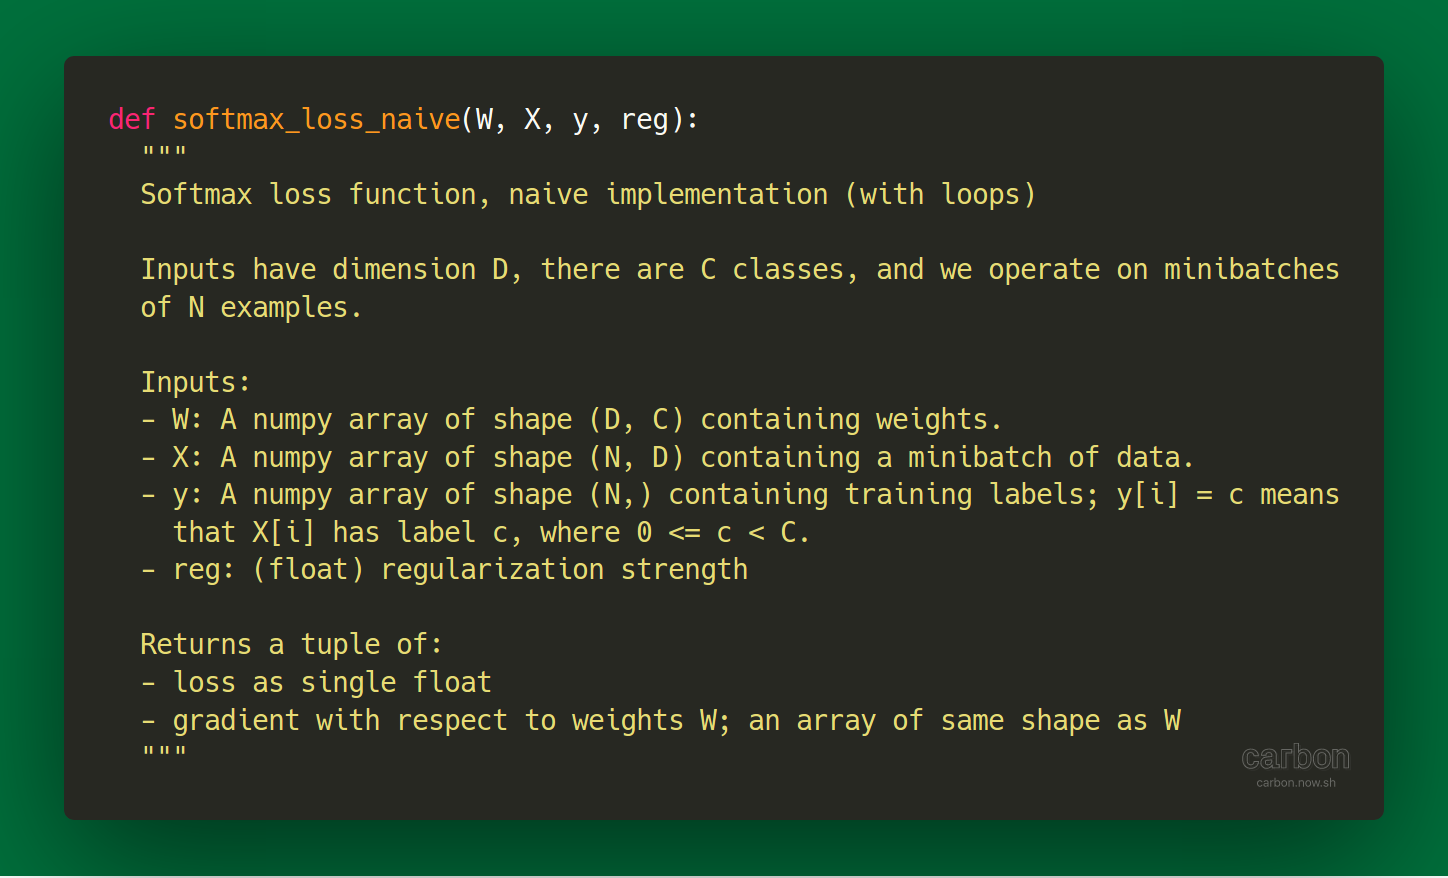
\includegraphics[width=\linewidth]{Resources/code.png}
\end{figure}
\footnote{\href{https://github.com/Rodas171315/PTI_4-DylanR-LaTeX_Beamer.git}{Github PTI 4}}

\end{frame}

\section{Ejercicio}
\begin{frame}
\frametitle{Resolución de Ejercicio}
La resolución del ejercicio con Beamer puede encontrarse en la presentación "Nota de Peter Norvig.pdf". Ver ahí.
\end{frame}

\end{document}